
\documentclass[landscape,a0paper,fontscale=.235]{xebaposter} % Adjust the font scale/size here

\usepackage{relsize}		% For \smaller

\usepackage{graphicx} % Required for including images
%\graphicspath{{figures/}} % Directory in which figures are stored

\usepackage{amsmath} % For typesetting math
\usepackage{amssymb} % Adds new symbols to be used in math mode

\usepackage{booktabs} % Top and bottom rules for tables
\usepackage{enumitem} % Used to reduce itemize/enumerate spacing
\usepackage{palatino} % Use the Palatino font
\usepackage[font=small,labelfont=bf]{caption} % Required for specifying captions to tables and figures

\usepackage{multicol} % Required for multiple columns
\setlength{\columnsep}{1.5em} % Slightly increase the space between columns
\setlength{\columnseprule}{0mm} % No horizontal rule between columns

\usepackage{tikz} % Required for flow chart
\usetikzlibrary{shapes,arrows} % Tikz libraries required for the flow chart in the template

\newcommand{\compresslist}{ % Define a command to reduce spacing within itemize/enumerate environments, this is used right after \begin{itemize} or \begin{enumerate}
\setlength{\itemsep}{1pt}
\setlength{\parskip}{0pt}
\setlength{\parsep}{0pt}
}

\definecolor{lightblue}{rgb}{0.145,0.6666,1} % Defines the color used for content box headers

\begin{document}

\begin{poster}
{
headerborder=closed, % Adds a border around the header of content boxes
colspacing=1em, % Column spacing
%bgColorOne=white, % Background color for the gradient on the left side of the poster
%bgColorTwo=white, % Background color for the gradient on the right side of the poster
background=none, % no background colour
borderColor=lightblue, % Border color
headerColorOne=black, % Background color for the header in the content boxes (left side)
headerColorTwo=lightblue, % Background color for the header in the content boxes (right side)
headerFontColor=white, % Text color for the header text in the content boxes
boxColorOne=white, % Background color of the content boxes
textborder=roundedleft, % Format of the border around content boxes, can be: none, bars, coils, triangles, rectangle, rounded, roundedsmall, roundedright or faded
eyecatcher=true, % Set to false for ignoring the left logo in the title and move the title left
headerheight=0.17\textheight, % Height of the header
headershape=roundedright, % Specify the rounded corner in the content box headers, can be: rectangle, small-rounded, roundedright, roundedleft or rounded
headerfont=\Large\bf\textsc, % Large, bold and sans serif font in the headers of content boxes
%textfont={\setlength{\parindent}{1.5em}}, % Uncomment for paragraph indentation
linewidth=1pt % Width of the border lines around content boxes
}
%----------------------------------------------------------------------------------------
%	TITLE SECTION 
%----------------------------------------------------------------------------------------
%
{
\setlength\fboxsep{0pt}
\setlength\fboxrule{0pt}
	\fbox{
		\begin{minipage}{8em}
			
\includegraphics[width=4.5em,height=4.5em]{cpl_logo.png}
			
\includegraphics[width=5em,height=4em]{mps_logo.png}
		\end{minipage}
	}
}
%{
\includegraphics[height=3em]{cpl_logo.png}} % First university/lab logo on the right
{\bf\textsc{\emph{restingIAF}: a reliable, automated method for quantifying Individual Alpha Frequency}\vspace{.2em}} % Poster title
{\smaller Andrew W Corcoran\textsuperscript{a,b} Phillip M Alday\textsuperscript{c,b} Matthias Schlesewsky\textsuperscript{b} Ina Bornkessel-Schlesewsky\textsuperscript{b}} % Author names
%{\includegraphics[height=5em]{cns_logo.jpg}} % Second university/lab logo on the right
{
\setlength\fboxsep{0pt}
\setlength\fboxrule{0pt}
	\fbox{
		\begin{minipage}{8em}
			
\includegraphics[width=4em,height=5em]{cnl.png}
			
\includegraphics[width=4em,height=5em]{unisa_logo.png}
		\end{minipage}
	}
}


%----------------------------------------------------------------------------------------
%	Intro
%----------------------------------------------------------------------------------------

\headerbox{Introduction}{name=intro,column=0,row=0}{

Donec non nisl a \textbf{arcu consequat} varius. Curabitur scelerisque mollis dolor, quis blandit lorem condimentum at. Pellentesque sed nibh vel \textbf{dolor} sagittis semper. 

\begin{enumerate}\compresslist
\item Feugiat vitae elit
\item bibendum ante sed lacinia eros in

\end{enumerate}

\vspace{0.3em} % When there are two boxes, some whitespace may need to be added if the one on the right has more content
}

%----------------------------------------------------------------------------------------
%	Problem
%----------------------------------------------------------------------------------------

\headerbox{Problem}{name=problem,column=1,row=0,bottomaligned=problem}{

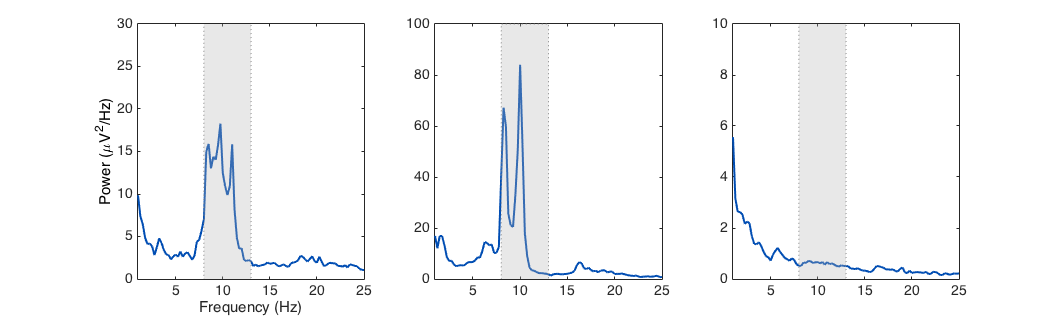
\includegraphics[width=\linewidth]{/figs/bad_pafs.png}
}


\end{poster}

\end{document}